% =====================================================================================
%  Paper 2 - growth-aware malignancy prediction on LUNA25.
%  Compile on Overleaf with pdfLaTeX + BibTeX (IEEEtran is built in there).
% =====================================================================================
\IfFileExists{IEEEtran.cls}{\documentclass[conference]{IEEEtran}}{%
  \documentclass[10pt,twocolumn]{article}\usepackage[margin=0.7in]{geometry}}
\usepackage{amsmath,amssymb}
\usepackage{graphicx}
\usepackage{booktabs}
\usepackage{multirow}
\usepackage{xcolor}
\usepackage{cite}
\usepackage[hidelinks]{hyperref}

\makeatletter
\providecommand{\IEEEauthorblockN}[1]{#1\\}
\providecommand{\IEEEauthorblockA}[1]{\small #1}
\@ifundefined{IEEEkeywords}{\newenvironment{IEEEkeywords}{\par\noindent\textbf{\textit{Index Terms}---}}{\par}}{}
\makeatother

\begin{document}

\title{Does Last Year's Scan Help? A Controlled, Reproducible Study of Growth-Aware Malignancy Prediction for Screen-Detected Lung Nodules on LUNA25}

\author{\IEEEauthorblockN{Abdullah Asim, Hussnain Khalid and Rabia Masood$^{*}$}
\IEEEauthorblockA{Department of Computer Sciences, Bahria University Lahore Campus, Lahore, Pakistan\\
abdullahasimnaawaz@gmail.com, hussnainkhalid421@gmail.com, rabiamasood.bulc@bahria.edu.pk\\
$^{*}$Corresponding author: Rabia Masood (rabiamasood.bulc@bahria.edu.pk)}}

\maketitle

\begin{abstract}
When a screen-detected lung nodule was also seen at an earlier round, radiologists look for growth before they decide on follow-up. Deep-learning risk models that use the prior CT exist, but they were trained on data that other groups cannot reuse, and their gain has not been separated from the effect of extra model capacity or checked against the size-and-growth rules used in practice. We study these questions on the public LUNA25 cohort (6{,}163 nodules, 555 malignant, 2{,}120 National Lung Screening Trial participants) with five-fold, patient-level cross-validation. A compact multi-scale 3D network (MSGF-Net) reaches an AUC of 0.875 on all nodules, above predicted size (0.830), Lung-RADS v2022 size categories (0.816) and a Brock model restricted to the variables available (0.843; all $p\le0.001$). At the sensitivity of Lung-RADS category 4A or higher it flags 917 benign nodules instead of 1{,}312, 30\% fewer. For the 2{,}401 nodules with a prior scan, a stacked model that adds the prior image raises the AUC from 0.904 to 0.932 ($p<0.001$), while a control network with identical capacity that sees the current scan twice stays at 0.905. Against Lung-RADS growth rules on these nodules the stacked model flags 45 instead of 76 benign nodules at equal sensitivity. The gain from the prior scan is concentrated in nodules of 8\,mm and larger (AUC 0.720 to 0.852 for 8--15\,mm, $p<0.001$), where management decisions are made, and is absent below 8\,mm. Decision-curve analysis shows a net benefit over size and over the single scan across clinically relevant thresholds. The code, splits and trained models are public so the comparison can be repeated.
\end{abstract}

\begin{IEEEkeywords}
lung cancer screening, malignancy prediction, nodule growth, longitudinal CT, Lung-RADS, Brock model, decision curve analysis, LUNA25, NLST
\end{IEEEkeywords}

% =====================================================================================
\section{Introduction}
Annual low-dose CT lowers lung-cancer mortality in heavy smokers~\cite{nlst2011}, yet most nodules it finds are benign. Management therefore depends on estimating, for each nodule, how likely it is to be cancer. Lung-RADS~\cite{lungrads2022} and the Fleischner recommendations~\cite{macmahon2017fleischner} rely mainly on size and on growth between scans, and the Brock (PanCan) model~\cite{mcwilliams2013brock} adds patient and morphological factors to the size of a nodule seen at baseline. Every false-positive category 4 result leads to extra CT, PET or biopsy, so a better risk estimate has a direct cost in patient harm and money.

Deep networks can read more from the image than its diameter. Ardila \emph{et al.}~\cite{ardila2019endtoend} and Venkadesh \emph{et al.}~\cite{venkadesh2021dl} showed that 3D models trained on NLST match or exceed radiologists and the Brock model, and Venkadesh \emph{et al.}~\cite{venkadesh2023prior} later found that adding the prior CT raised the AUC of their model on two European screening cohorts. These results come from data obtained under controlled access, with code and trained models that are not public, and they leave three practical questions open. How much of the gain from a prior scan is due to the prior image itself, and how much to a larger model? Is a learned temporal network needed, or does a simple growth formula do as well? And how does the result compare with the size-and-growth rules radiologists already apply?

The LUNA25 challenge~\cite{luna25} released pathology-confirmed NLST nodules together with the screening round and lesion identity. This makes it possible, for the first time on fully public data, to answer these questions in a way others can repeat. We do so with five-fold, patient-level cross-validation and participant-level bootstrap tests.

Our contributions are:
\begin{enumerate}
\item A single-scan 3D model that beats predicted size, Lung-RADS size categories and a reduced Brock model on all 6{,}163 LUNA25 nodules, with 30\% fewer benign nodules flagged at the sensitivity of Lung-RADS 4A+.
\item A controlled measurement of what the prior scan adds: a growth formula, a learned temporal network (TG-MSGF) and their combination are compared with a no-prior control of identical capacity, so the gain can be attributed to the earlier image.
\item An analysis of where the gain occurs. It is concentrated in nodules of 8\,mm and above, and it reduces benign flags against Lung-RADS growth rules by 41\% at equal sensitivity.
\item Calibration and decision-curve analysis, which show the models are usable as probabilities and give a net benefit over size-based rules.
\item Public code, patient-level splits and trained models.
\end{enumerate}

% =====================================================================================
\section{Related Work}
\textbf{Clinical models.} Lung-RADS v2022 assigns solid nodules to categories by diameter at baseline and by growth of more than 1.5\,mm at follow-up~\cite{lungrads2022}. The Brock model~\cite{mcwilliams2013brock} combines age, sex, family history, emphysema, nodule size, type, upper-lobe location, nodule count and spiculation in a logistic regression, and is recommended by several guidelines for baseline nodules.

\textbf{Image-based risk.} Early work on LIDC-IDRI~\cite{armato2011lidc} predicted radiologists' subjective malignancy ratings, which are not pathology labels. NLST-based studies use confirmed outcomes. Ardila \emph{et al.}~\cite{ardila2019endtoend} reported an AUC of 0.944 on 6{,}716 NLST cases with a whole-volume model. Venkadesh \emph{et al.}~\cite{venkadesh2021dl} trained a nodule-level model on NLST and reached an AUC of 0.93 on Danish screening data, against 0.90 for the PanCan (Brock) model. Sybil~\cite{mikhael2023sybil} predicts future lung-cancer risk for the whole scan rather than for a given nodule. In the LUNA25 challenge the best algorithm reached an AUC of 0.78 on 5--15\,mm indeterminate nodules from three European trials, against 0.70 for 65 radiologists~\cite{peeters2026luna25}; prior scans were not part of that task.

\textbf{Using the prior scan.} Gao \emph{et al.}~\cite{gao2019distanced} added the time between scans to the gates of an LSTM over serial CT. Ardila \emph{et al.}~\cite{ardila2019endtoend} showed that their model, given a prior CT, performed on par with radiologists who also had it. Venkadesh \emph{et al.}~\cite{venkadesh2023prior} encoded current and prior nodule patches with a shared network and reported an AUC rise from 0.85 to 0.91 and from 0.89 to 0.94 on two external cohorts, with the PanCan model at 0.63--0.64 on the same cancer-enriched sets. Our TG-MSGF follows the same shared-encoder idea. What we add is a no-prior control with identical parameters, a comparison with a transparent growth formula and with Lung-RADS growth rules, a breakdown by size group, and an evaluation on public data that others can rerun.

\textbf{Backbone.} The encoder is MSGF-Net, which we developed for nodule false-positive reduction on LUNA16~\cite{setio2017luna16,asim2026msgf}. It reads a 32\,mm and a 48\,mm view in three Hounsfield-unit windows through residual squeeze-excitation blocks~\cite{hu2018se,he2016resnet} and fuses the two scales with a learned gate, in the spirit of multi-scale contextual 3D networks~\cite{dou2017multilevel}.

% =====================================================================================
\section{Data}
LUNA25 contains 6{,}163 nodules with known position in 4{,}069 low-dose CT scans of 2{,}120 NLST participants (mean age $63.3\pm5.2$ years); 555 nodules (9.0\%) are malignant. We extracted a 48\,mm cube at 1\,mm spacing around each nodule.

\textbf{Source and licence.} We used the public LUNA25 training and development set~\cite{luna25}, drawn from NLST participants enrolled in 2002--2004 at 33 US centres. The images (4{,}069 volumes in MetaImage \texttt{.mha} format, 221.1\,GB) are released under CC BY 4.0 (Zenodo record 14223624), and the annotation file under CC BY-NC 4.0 (DOI 10.5281/zenodo.14673658), which permits the non-commercial research use made here; no separate permission is required. For each nodule the file gives the series identifier, world coordinates, malignancy label, participant identifier, an identifier that links the same lesion across screening rounds, age and sex.

\textbf{Splits.} Participants were divided into five folds with a stratified group split (seed 2026), so that all nodules and scans of one person fall in one fold. In the first experiments fold~0 is the test set (1{,}241 nodules, 111 malignant, 424 participants), fold~1 the validation set and folds 2--4 the training set. The validation fold is used only for early stopping, Platt calibration~\cite{platt1999} and fitting the small combination models.

\textbf{Pairs.} Linking annotations of the same lesion across screening rounds gives 2{,}401 current--prior pairs from 3{,}762 lesions; the median interval is 1.0 year, and no lesion changes label between rounds. Of the pairs, 207 are malignant. Pairs inherit the participant's fold.

% =====================================================================================
\section{Methods}
\begin{figure*}[t]
\centering
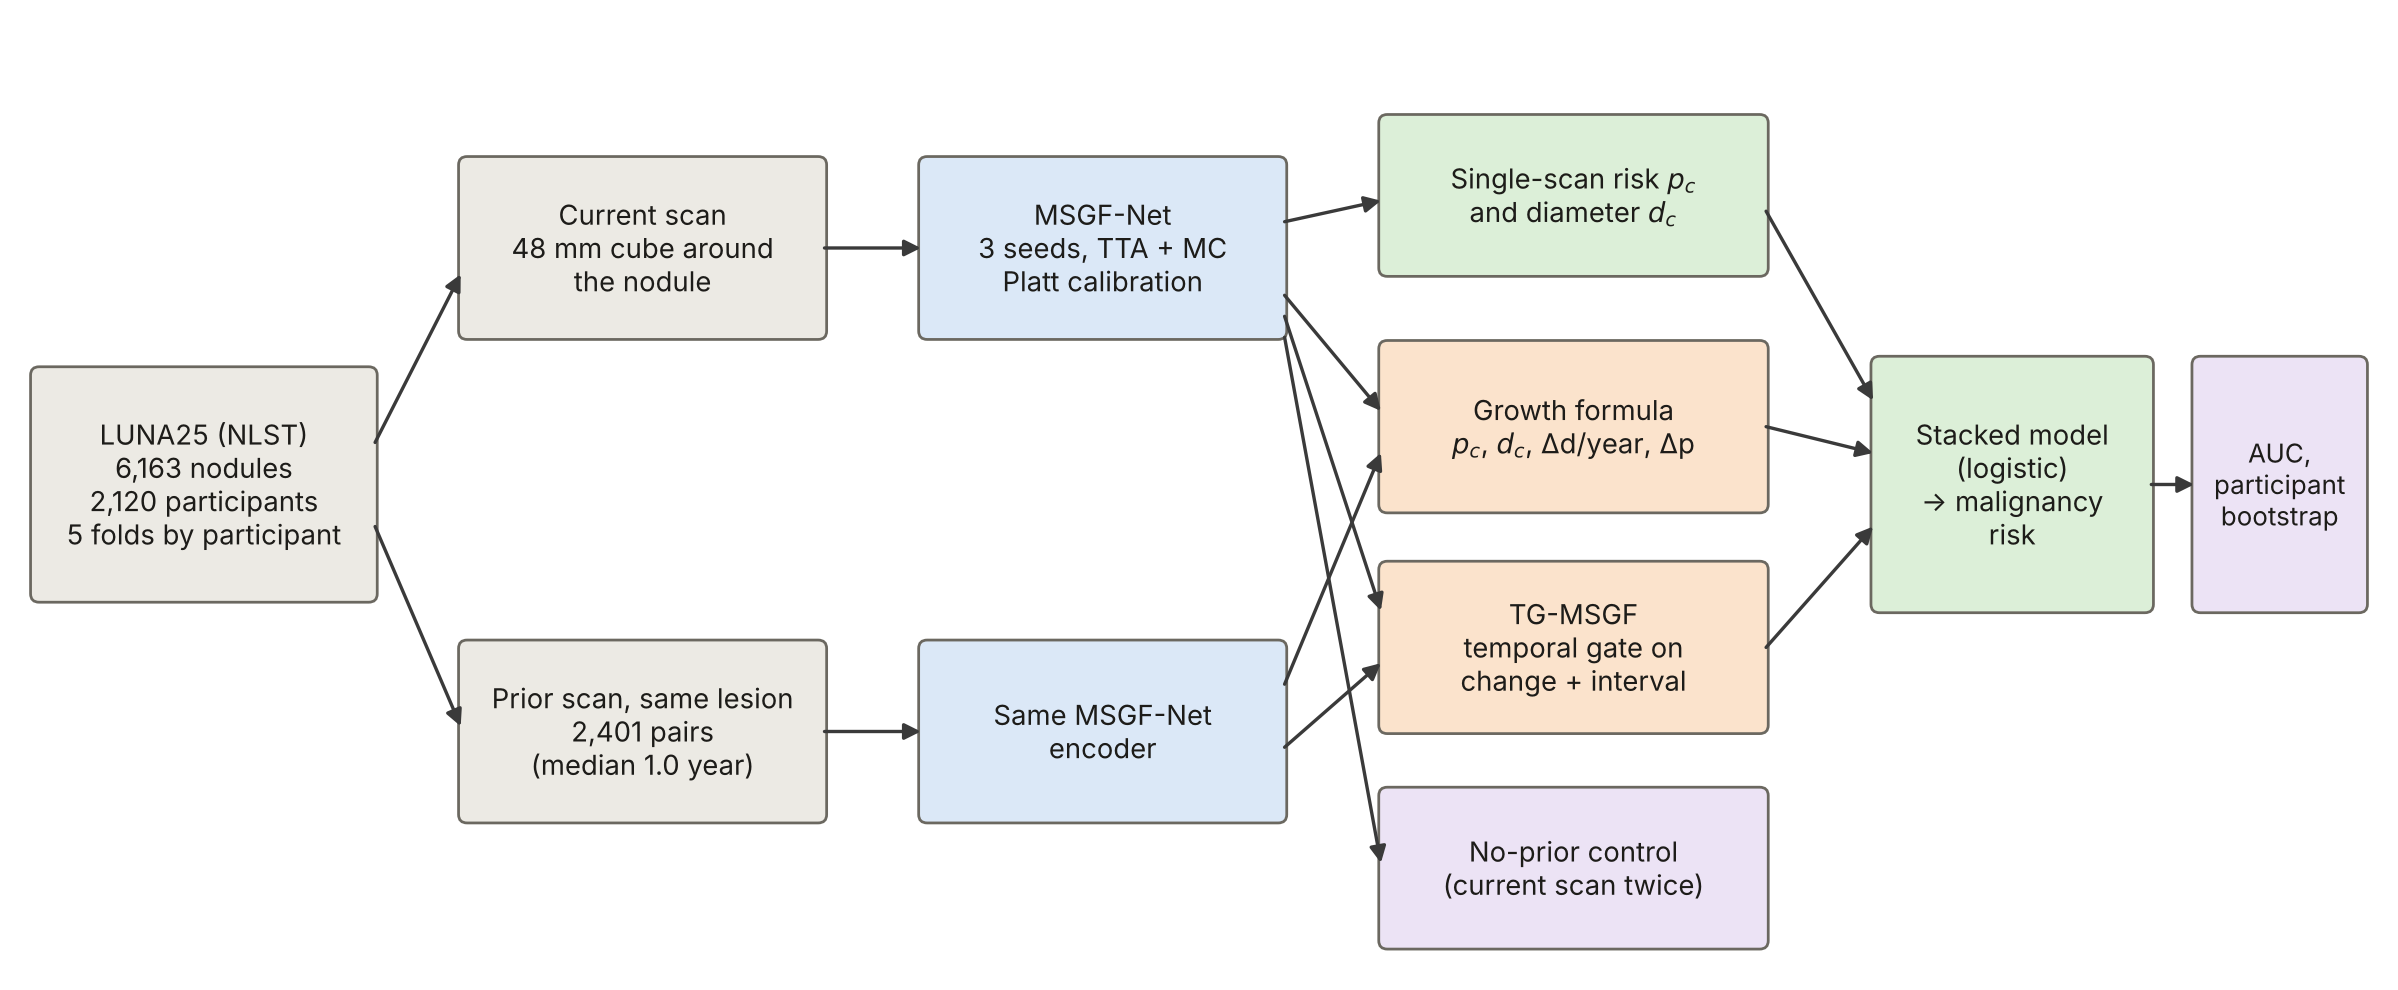
\includegraphics[width=0.92\textwidth]{figures/paper2_method.png}
\caption{Study design. Current and prior 48\,mm nodule cubes are encoded by MSGF-Net; single-scan risk, a growth formula, the temporal model TG-MSGF and a no-prior control are compared, and a stacked model combines them. All models are evaluated on held-out participants.}
\label{fig:method}
\end{figure*}

\subsection{Single-scan malignancy model}
We train MSGF-Net from random initialisation to predict malignancy from one 48\,mm patch, using the recipe of our detection work: focal loss~\cite{lin2017focal}, AdamW with cosine decay, class-balanced sampling and flip, rotation, shift and intensity augmentation. Three seeds are trained and their calibrated outputs averaged. At test time each nodule is scored on eight flipped views with Monte-Carlo dropout in the head~\cite{gal2016dropout}. We also tried initialising from the LUNA16 detection weights and fusing the network output with age by logistic regression.

\subsection{Using the prior scan}
\textbf{Growth formula.} A logistic regression on four standardised features: the current single-scan risk, the current predicted diameter, the change in diameter per year and the change in single-scan risk between the two rounds.

\textbf{TG-MSGF.} A shared MSGF-Net encoder, initialised from the single-scan model, maps the current and prior patches to descriptors $z_c$ and $z_p$. With the change $d=z_c-z_p$ and the interval $\Delta t$ in years, a gate
\begin{equation}
\beta=\sigma\!\left(W_2\,\mathrm{ReLU}(W_1[z_c,d,\Delta t])\right)
\end{equation}
decides per channel how much of the change to pass on, and the risk is predicted from $[z_c,\ \beta\odot d]$ by a two-layer head with dropout. The encoder is fine-tuned at one tenth of the head's learning rate (20 epochs of 3{,}000 pairs, early stopping on validation AUC, three seeds).

\textbf{No-prior control.} The same network is trained with the prior patch replaced by the current one and $\Delta t=0$. It has exactly the parameters of TG-MSGF but no access to the earlier image, so any difference between the two isolates the information in the prior scan.

\textbf{Stacked model.} A logistic regression, fitted on the validation fold, combines single-scan risk, TG-MSGF risk, diameter change per year and risk change.

\subsection{Clinical reference models}
LUNA25 gives no measured diameters, so all size-based references use the diameter predicted by the LUNA16 MSGF-Net (median 6.2\,mm, IQR 5.1--8.5\,mm). Both arms therefore see the same patch.

\textbf{Predicted size.} A logistic regression on predicted diameter, fitted on the validation fold.

\textbf{Lung-RADS v2022.} For all nodules we apply the baseline rules for solid nodules: category 2 below 6\,mm, 3 for 6 to $<$8\,mm, 4A for 8 to $<$15\,mm and 4B from 15\,mm. For nodules with a prior scan we apply the follow-up rules: growth is an increase in mean diameter of more than 1.5\,mm within 12 months; a growing nodule is 4A below 8\,mm and 4B from 8\,mm, and a nodule that does not grow is category 2. The ordered category is used as a score for the AUC, and category 4A or higher as the positive call.

\textbf{Reduced Brock model.} We apply the published coefficients of the full Brock model~\cite{mcwilliams2013brock} without refitting. Age, sex, predicted size and the number of annotated nodules in the scan are taken from the data; family history, emphysema, nodule type, upper-lobe location and spiculation are not available in LUNA25 and are set to their reference values (no, no, solid, not upper lobe, not spiculated). This is a lower bound on what the full model could do and is reported as such.

\subsection{Evaluation}
Fold $k$ is the test set, fold $k{+}1$ the validation set and the other three folds the training set; every model is calibrated on its own validation fold, and the five test folds are pooled so that each nodule is scored by a model that never saw its owner. The primary measure is the AUC. Confidence intervals and two-sided $p$-values for paired differences come from 2{,}000 bootstrap resamples of participants, not of nodules, because nodules of one person are correlated. We also report average precision (AP), specificity at 95\% sensitivity, the number of benign nodules flagged at the operating point of Lung-RADS 4A+, calibration (Brier score, expected calibration error over ten quantile bins, calibration slope) and decision curves, which give the net benefit of acting on a model at each risk threshold~\cite{vickers2006dca}.

% =====================================================================================
\section{Results}
\subsection{Single scan versus size on the first split}
Table~\ref{tab:single} shows the held-out results of fold~0. The three-seed ensemble reaches an AUC of 0.900, 0.044 above predicted size ($p=0.001$). The three seeds individually give 0.900, 0.892 and 0.888 (mean $0.893\pm0.006$), so the result is not driven by one run; Table~\ref{tab:single} lists the first seed, which also had the highest validation AUC. Adding age changed nothing ($\Delta<0.001$, $p=0.96$), and starting from the LUNA16 detection weights was, if anything, worse (0.878, $p=0.061$ against the ensemble): features learned to separate nodules from vessels do not carry over directly to separating cancers from benign nodules.

\begin{table}[t]
\centering
\caption{Malignancy prediction on the held-out fold (1{,}241 nodules, 111 malignant, 424 participants).}
\label{tab:single}
\setlength{\tabcolsep}{4pt}
\resizebox{\columnwidth}{!}{%
\begin{tabular}{lccc}
\toprule
Model & AUC (95\% CI) & AP & Sens./Spec. \\
\midrule
Predicted size only & 0.856 (0.816--0.894) & 0.428 & 0.739 / 0.810 \\
MSGF-Net, LUNA16 init. & 0.878 (0.841--0.912) & 0.457 & 0.820 / 0.788 \\
MSGF-Net, first seed & 0.900 (0.864--0.934) & 0.548 & 0.874 / 0.689 \\
MSGF-Net, 3 seeds & \textbf{0.900} (0.861--0.934) & \textbf{0.576} & 0.856 / 0.719 \\
\quad + size + age & 0.900 (0.862--0.933) & 0.570 & 0.865 / 0.732 \\
\bottomrule
\end{tabular}}
\end{table}

Size explains much of the overall AUC because large nodules are more often malignant. Fig.~\ref{fig:size} removes that effect by evaluating within diameter groups. Inside every group size alone is close to chance (0.50--0.65), whereas the network stays between 0.65 and 0.84. The 6--8\,mm group, where follow-up decisions are hardest, is also where both models are weakest; the $<$6\,mm group has only six cancers and a very wide interval.

\begin{figure}[t]
\centering
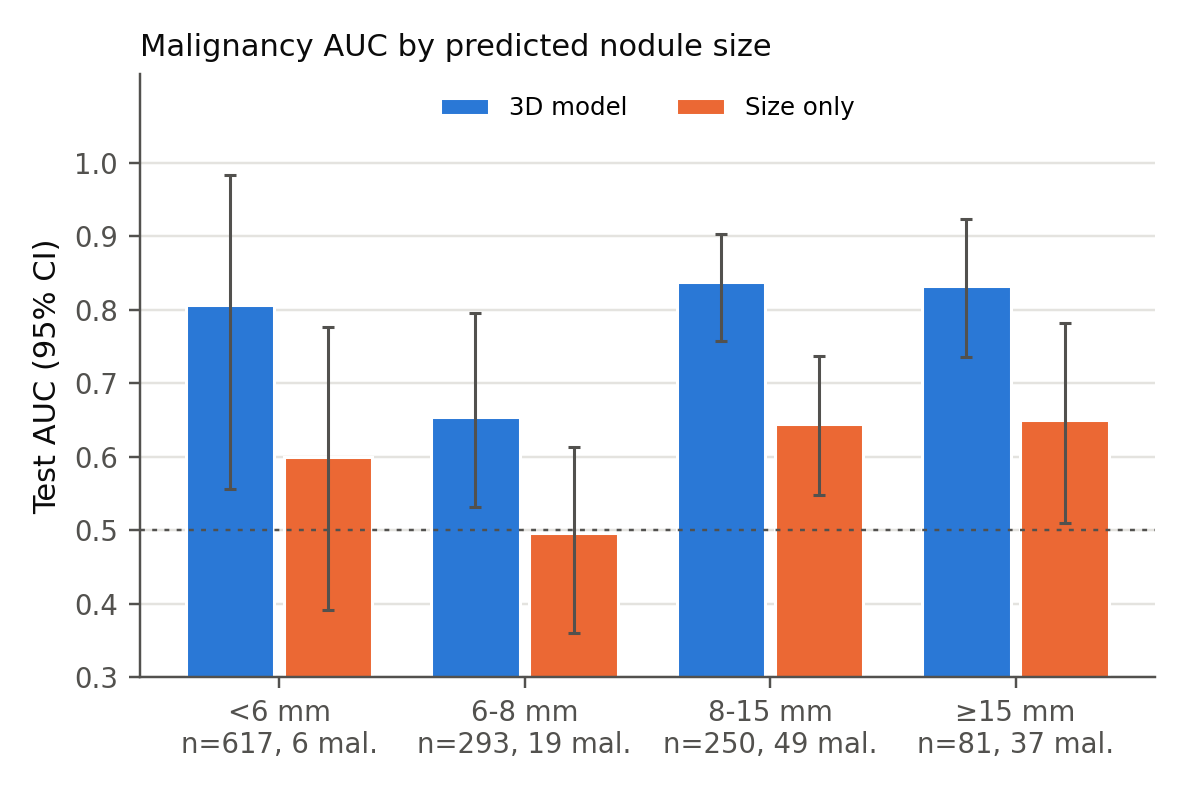
\includegraphics[width=\columnwidth]{figures/auc_by_size.png}
\caption{AUC within predicted-diameter groups (held-out fold). Error bars: participant-level bootstrap 95\% CI.}
\label{fig:size}
\end{figure}

\subsection{Comparison with clinical models}
Table~\ref{tab:clinical} gives the pooled five-fold results against the clinical references. On all 6{,}163 nodules the network reaches 0.875, ahead of the reduced Brock model by 0.032 ($p=0.001$), of predicted size by 0.045 and of Lung-RADS size categories by 0.059 (both $p<0.001$).

The AUC gap translates into fewer unnecessary work-ups. Lung-RADS 4A+ finds 75.5\% of cancers and flags 1{,}312 of the 5{,}608 benign nodules. At the same sensitivity the network flags 917, which is 395 (30\%) fewer; at the same specificity it finds 84.0\% of cancers instead of 75.5\%. At 95\% sensitivity, the level a screening programme would aim for, the network clears 54.8\% of benign nodules (95\% CI 49.7--61.9), against 46.4\% for the reduced Brock model and 38.6\% for size.

\begin{table}[t]
\centering
\caption{Five-fold cross-validation against clinical references (pooled test predictions). $\Delta$ and $p$: paired bootstrap against the network (top) or the stacked model (bottom). Spec@95: specificity at 95\% sensitivity.}
\label{tab:clinical}
\setlength{\tabcolsep}{3pt}
\resizebox{\columnwidth}{!}{%
\begin{tabular}{lcccc}
\toprule
Model & AUC (95\% CI) & $\Delta$ & $p$ & Spec@95 \\
\midrule
\multicolumn{5}{l}{\emph{All nodules (6{,}163; 555 malignant)}}\\
Lung-RADS v2022 (size) & 0.816 (0.795--0.837) & $-0.059$ & $<$0.001 & -- \\
Predicted size & 0.830 (0.808--0.851) & $-0.045$ & $<$0.001 & 0.386 \\
Brock, reduced & 0.843 (0.821--0.862) & $-0.032$ & 0.001 & 0.464 \\
MSGF-Net, single scan & \textbf{0.875} (0.857--0.892) & -- & -- & \textbf{0.548} \\
\midrule
\multicolumn{5}{l}{\emph{Nodules with a prior scan (2{,}401; 207 malignant)}}\\
Lung-RADS v2022 (growth) & 0.771 (0.738--0.807) & $-0.161$ & $<$0.001 & -- \\
Brock, reduced & 0.866 (0.837--0.894) & $-0.066$ & $<$0.001 & 0.498 \\
Stacked, with prior & \textbf{0.932} (0.912--0.950) & -- & -- & \textbf{0.646} \\
\bottomrule
\end{tabular}}
\end{table}

\subsection{Adding the prior scan}
Table~\ref{tab:cv} gives the pooled results for the nodules with a prior scan. Every method that sees the earlier image improves on the single scan. The growth formula adds 0.021 ($p=0.003$), TG-MSGF 0.013 ($p=0.043$) and the stacked model 0.029 ($p<0.001$), which is also better than the formula alone ($p=0.027$). The no-prior control is no better than the single scan, and TG-MSGF beats it by 0.012 ($p=0.012$). The per-fold standard deviation of the stacked model (0.011) is half that of the single scan (0.021).

\begin{table}[t]
\centering
\caption{Five-fold patient-level cross-validation on nodules with a prior scan (2{,}401; 207 malignant). $p$: paired bootstrap against the single scan.}
\label{tab:cv}
\setlength{\tabcolsep}{3.5pt}
\resizebox{\columnwidth}{!}{%
\begin{tabular}{lcccc}
\toprule
Model & AUC (95\% CI) & Fold mean$\pm$SD & AP & $p$ \\
\midrule
Single scan & 0.904 (0.881--0.924) & $0.907\pm0.021$ & 0.493 & -- \\
No-prior control & 0.905 (0.883--0.924) & $0.908\pm0.008$ & 0.475 & \\
TG-MSGF & 0.917 (0.895--0.936) & $0.924\pm0.014$ & 0.617 & 0.043 \\
Growth formula & 0.924 (0.904--0.943) & $0.927\pm0.012$ & 0.655 & 0.003 \\
Stacked & \textbf{0.932} (0.912--0.950) & $0.936\pm0.011$ & \textbf{0.686} & $<$0.001 \\
\bottomrule
\end{tabular}}
\end{table}

The gains are larger in average precision than in AUC (0.49 to 0.69 for the stacked model). With a 9\% prevalence, average precision rewards a model that ranks the few cancers at the very top, and growth is the feature that pushes a growing nodule above stable ones of similar appearance.

Against the Lung-RADS follow-up rules the difference is large. Lung-RADS calls 57.5\% of these cancers and 76 benign nodules category 4A or higher. At that sensitivity the stacked model flags 45 benign nodules, 41\% fewer; at the Lung-RADS specificity (96.5\%) it finds 66.2\% of cancers. Many cancers in this set are already large at the earlier round and grow slowly, which a 1.5\,mm growth threshold on its own misses.

\subsection{Where the prior scan helps}
Table~\ref{tab:sizegroups} splits the nodules with a prior scan by current size. Below 8\,mm the prior scan adds nothing measurable: the single-scan AUC is already about 0.87--0.90 and the differences are within noise. From 8\,mm upward, where a single scan is much weaker (0.72 and 0.76) and where Lung-RADS calls for PET-CT or tissue sampling, the stacked model gains 0.13 and 0.12 ($p<0.001$ and $p=0.002$). The overall gain of 0.029 is therefore an average of no change in small nodules and a large change in the nodules that drive invasive work-up.

\begin{table}[t]
\centering
\caption{AUC of the single scan and the stacked model with prior scan, by current predicted diameter (nodules with a prior scan, pooled five-fold predictions).}
\label{tab:sizegroups}
\setlength{\tabcolsep}{4pt}
\resizebox{\columnwidth}{!}{%
\begin{tabular}{lcccccc}
\toprule
Size & $n$ & Mal. & Single & Stacked & $\Delta$ & $p$ \\
\midrule
$<$6\,mm & 1{,}111 & 9 & 0.903 & 0.912 & $+0.009$ & 0.70 \\
6--8\,mm & 643 & 36 & 0.871 & 0.866 & $-0.005$ & 0.81 \\
8--15\,mm & 497 & 96 & 0.720 & \textbf{0.852} & $+0.131$ & $<$0.001 \\
$\ge$15\,mm & 150 & 66 & 0.756 & \textbf{0.880} & $+0.124$ & 0.002 \\
\bottomrule
\end{tabular}}
\end{table}

\subsection{Calibration and clinical utility}
After Platt scaling on the validation fold the single-scan network is well calibrated on the pooled test folds: expected calibration error 0.008, calibration slope 0.91 and Brier score 0.063, against 0.071 for size (Fig.~\ref{fig:cal}). On nodules with a prior scan the stacked model has a slope of 1.02 and a Brier score of 0.044, against 0.057 for the single scan. The reduced Brock model ranks reasonably but predicts a mean risk of 2.9\% for a 9.0\% prevalence. This is expected when the factors that raise risk are set to their reference values, and it is why we compare it by AUC and specificity rather than by its probabilities.

Fig.~\ref{fig:dca} shows decision curves. On all nodules the network has a higher net benefit than size and the reduced Brock model at every threshold from 1\% to 30\%, and it is better than referring every nodule above about 2\%. For nodules with a prior scan the stacked and single-scan curves coincide below about 8\%; above it the stacked model keeps a clearly higher net benefit, which matches the size-group result: the prior scan matters most for the higher-risk nodules where an intervention is considered.

\begin{figure}[t]
\centering
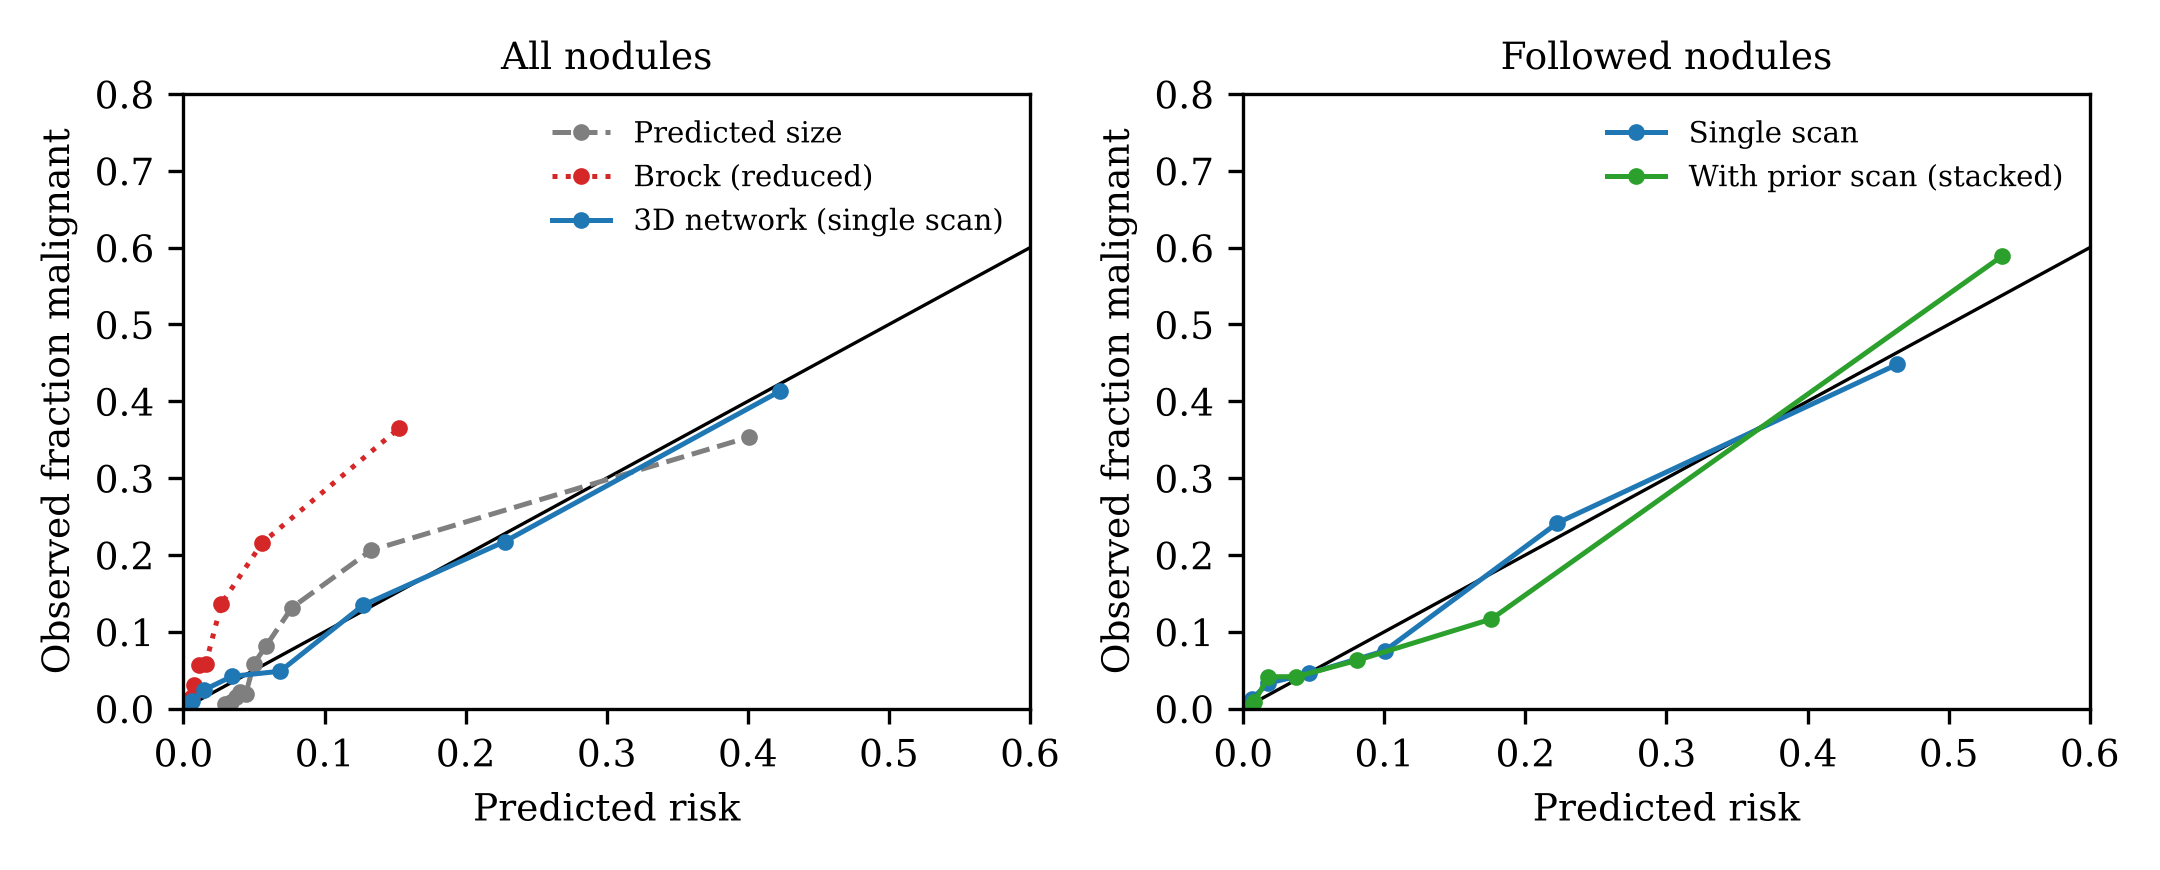
\includegraphics[width=\columnwidth]{figures/calibration.png}
\caption{Calibration of pooled five-fold predictions (deciles of predicted risk). Left: all nodules; right: nodules with a prior scan.}
\label{fig:cal}
\end{figure}

\begin{figure}[t]
\centering
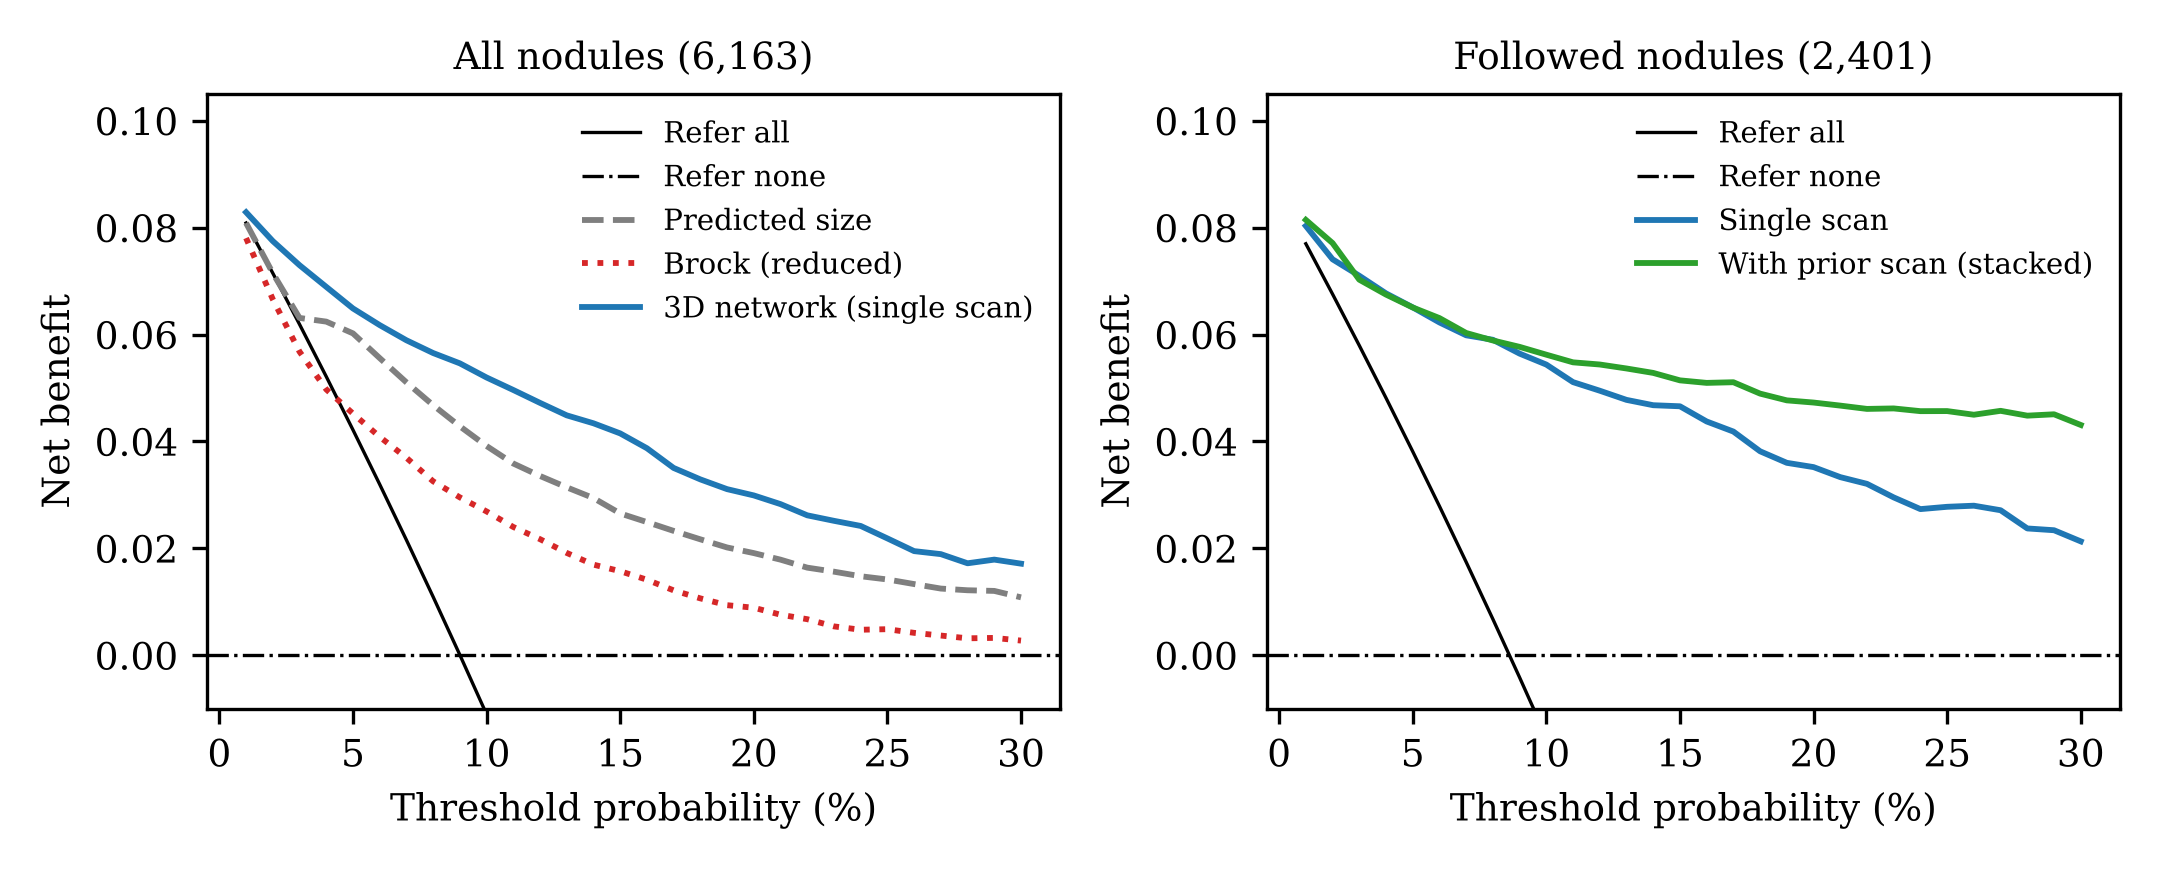
\includegraphics[width=\columnwidth]{figures/dca.png}
\caption{Decision curves~\cite{vickers2006dca} for pooled five-fold predictions. Net benefit is the fraction of true positives minus the fraction of false positives weighted by the odds of the threshold.}
\label{fig:dca}
\end{figure}

\subsection{A single split is not enough}
On fold~0 alone (475 pairs, 43 malignant), the ordering is the same: single scan 0.922, TG-MSGF 0.921, growth formula 0.933 and stacked 0.936 (Fig.~\ref{fig:roc2}). None of these differences reaches significance (stacked versus single, $p=0.108$), although TG-MSGF again beats its no-prior control ($p=0.003$). Had we stopped at the first split, we would have concluded that the prior scan does not help. Fold-to-fold variation in the single-scan AUC on paired nodules (0.874 to 0.927) is as large as the effect being measured, which is why we consider cross-validation essential for this question.

\begin{figure}[t]
\centering
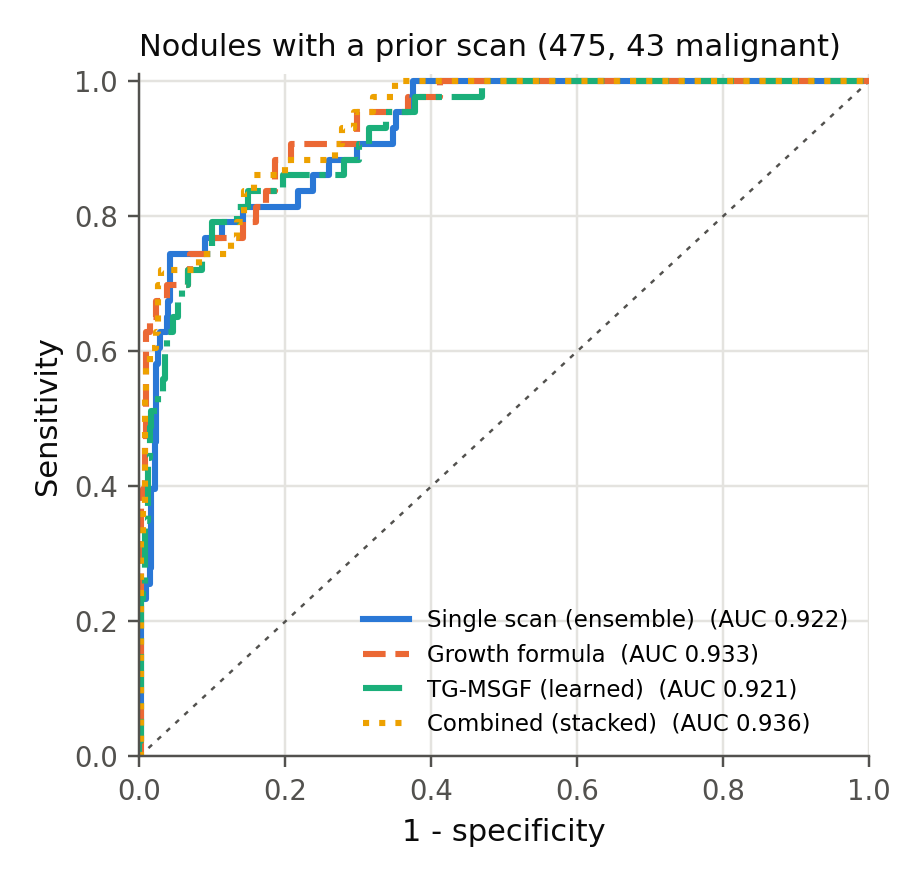
\includegraphics[width=0.85\columnwidth]{figures/roc_temporal.png}
\caption{ROC curves on the held-out fold for nodules with a prior scan.}
\label{fig:roc2}
\end{figure}

\subsection{What the models use}
The fitted coefficients of the growth formula (standardised features) are 2.73 for the current risk, $-0.29$ for current diameter, 0.88 for diameter change per year and 0.42 for risk change: once the image-based risk is known, current size adds little, but growth adds a lot. In the stacked model, single-scan risk, TG-MSGF risk and diameter growth all keep positive weights (1.19, 1.31 and 0.81), so the learned temporal features and the explicit growth term carry partly different information. The mean gate value of TG-MSGF is only slightly higher for malignant than for benign pairs (0.53 versus 0.52) and correlates weakly with diameter growth (Spearman 0.12), so the gate should not be read as a growth detector.

% =====================================================================================
\section{Discussion}
The prior scan helps, and on public data the size of the help agrees with what Venkadesh \emph{et al.}~\cite{venkadesh2023prior} found on controlled-access NLST data and external European cohorts: in both studies the AUC rises by a few hundredths overall. Our controlled design adds three things. First, the gain belongs to the prior image: a network with the same parameters that sees the current scan twice gains nothing. Second, a transparent four-feature growth formula captures most of the benefit, and the learned temporal network adds a smaller, significant increment when the two are combined; for deployment this is convenient, because the formula needs only the single-scan model run on both scans. Third, the average hides where the gain is. It is concentrated in nodules of 8\,mm and above, the ones that Lung-RADS sends to PET-CT, biopsy or short-interval follow-up, and absent in small nodules, which are already handled well from one scan.

Against the rules used in practice the improvement is larger than the AUC differences suggest. Compared with Lung-RADS, the single-scan model would spare about three in ten benign nodules from a category 4 call at the same sensitivity, and with the prior scan about four in ten. These are retrospective estimates on predicted diameters and should be read as the size of the opportunity rather than as a clinical result.

Effect sizes of 0.01--0.03 AUC are of the same order as the variation between test folds. Results on one split with a few dozen cancers, which are common in this area, can point either way; our own first split did. Cross-validation with participant-level resampling should be the norm for longitudinal nodule studies.

Table~\ref{tab:compare} places our results next to published malignancy studies. The AUCs come from different cohorts, inputs and case mixes and are not directly comparable. In particular, the LUNA25 challenge test set contains only indeterminate 5--15\,mm nodules from European trials, a harder task on which the best algorithm reached 0.78~\cite{peeters2026luna25}; our cross-validated results include nodules of all sizes from NLST and probably overestimate performance on external data.

\begin{table}[t]
\centering
\caption{Comparison with published malignancy-risk studies. AUCs come from different cohorts and test sets and are not directly comparable.}
\label{tab:compare}
\small\setlength{\tabcolsep}{3pt}
\begin{tabular}{@{}p{2.35cm}p{2.85cm}ccc@{}}
\toprule
Study & Data and test & Prior & Public & AUC\\
\midrule
Ardila \emph{et al.}~\cite{ardila2019endtoend} & NLST, 6{,}716 test cases & yes & no & 0.944\\
Venkadesh 2021~\cite{venkadesh2021dl} & DLCST, 883 nodules & no & no & 0.93\\
Venkadesh 2023~\cite{venkadesh2023prior} & DLCST, MILD (129, 126 nodules) & yes & no & 0.91, 0.94\\
LUNA25 challenge, best AI~\cite{peeters2026luna25} & 468 external 5--15\,mm nodules & no & yes & 0.78\\
\midrule
Ours, single scan & 5-fold CV, 6{,}163 nodules & no & yes & 0.875\\
Ours, stacked & 5-fold CV, 2{,}401 followed nodules & yes & yes & 0.932\\
\bottomrule
\end{tabular}
\end{table}

\textbf{Limitations.} All data come from one trial, with one scanner generation and a single population; an external cohort is needed. Size, growth and the Lung-RADS categories use predicted rather than measured diameter, and Lung-RADS is applied only with its rules for solid nodules. The Brock model is reduced to the variables LUNA25 provides, so it understates the full model; its probabilities are too low for this reason. Pairs exist only for nodules seen in two rounds, which favours slow-growing lesions; cancers that appear between screens are not represented. Uncertainty estimates of the single-scan model did not help in triage: referring the 10\% most uncertain nodules lowered the remaining AUC slightly compared with referring a random 10\% (0.903 versus 0.919), so we do not claim a use for uncertainty in this task. Finally, the system is a research prototype for decision support, not a diagnostic device.

\section{Conclusion}
On public NLST data with patient-level cross-validation, a compact 3D network predicts nodule malignancy better than size, Lung-RADS categories and a reduced Brock model (AUC 0.875 versus 0.816--0.843) and flags 30\% fewer benign nodules than Lung-RADS 4A+ at the same sensitivity. Adding the prior-year scan raises the AUC for followed nodules from 0.904 to 0.932; a matched no-prior control shows that the gain comes from the earlier image, and a breakdown by size shows that it is concentrated in nodules of 8\,mm and above. A simple growth formula provides most of the gain and a learned temporal model adds to it. Single-split experiments were too small to show these effects reliably.

\textbf{What this work overcomes, and future work.} Earlier studies of the prior scan used data and models that others cannot reuse and did not separate the prior image from model capacity or compare against growth rules. This study does both on public data, so others can repeat it. Future work will validate the models on an external cohort, including the LUNA25 hidden test set, replace predicted diameter with measured volume and volume-doubling time, add the missing Brock variables where they can be read from the image (nodule type, location, spiculation, emphysema), and test whether the uncertainty estimate can support triage when the model is trained for longer.

\section*{Author Contributions}
A. Asim: conceptualization, methodology, software, experiments, formal analysis, visualization and writing of the original draft. H. Khalid: application testing, and writing (review and editing). R. Masood: supervision, project administration, and writing (review and editing). All authors read and approved the final manuscript.

\section*{Funding}
This research received no external funding. Computing resources were provided by the Department of Computer Sciences, Bahria University Lahore Campus.

\section*{Conflict of Interest}
The authors declare no conflict of interest.

\section*{Data and Code Availability}
LUNA25 is publicly available~\cite{luna25} at \url{https://luna25.grand-challenge.org} (images: CC BY 4.0; annotations: CC BY-NC 4.0). Code (including \texttt{paper2\_extra.py} for the clinical comparisons, calibration and decision curves), split definitions, the three trained single-scan models, experiment logs and all result files are available at \url{https://github.com/mabdullah52/FYP-Project}.

\section*{Declaration of Generative AI Use}
During the preparation of this work the authors used an AI assistant (Claude, Anthropic) to help write code and to edit the language of the manuscript. The authors reviewed and edited all content and take full responsibility for the publication.

\IfFileExists{IEEEtran.bst}{\bibliographystyle{IEEEtran}}{\bibliographystyle{unsrt}}
\bibliography{refs}

\end{document}
